\clearpage

\section*{三、结果与分析}

\subsection*{1. 手动曲线与峰位判定}

以实测加速电压为横轴、板极电流为纵轴作图。完整电流曲线有周期性峰谷，不能用一条直线拟合整条电流—电压曲线；课堂要求的线性拟合是对“峰序—峰位”进行的。图中采样点间的线段仅用于显示走势，没有改变实测数据。

\begin{figure}[H]
\centering
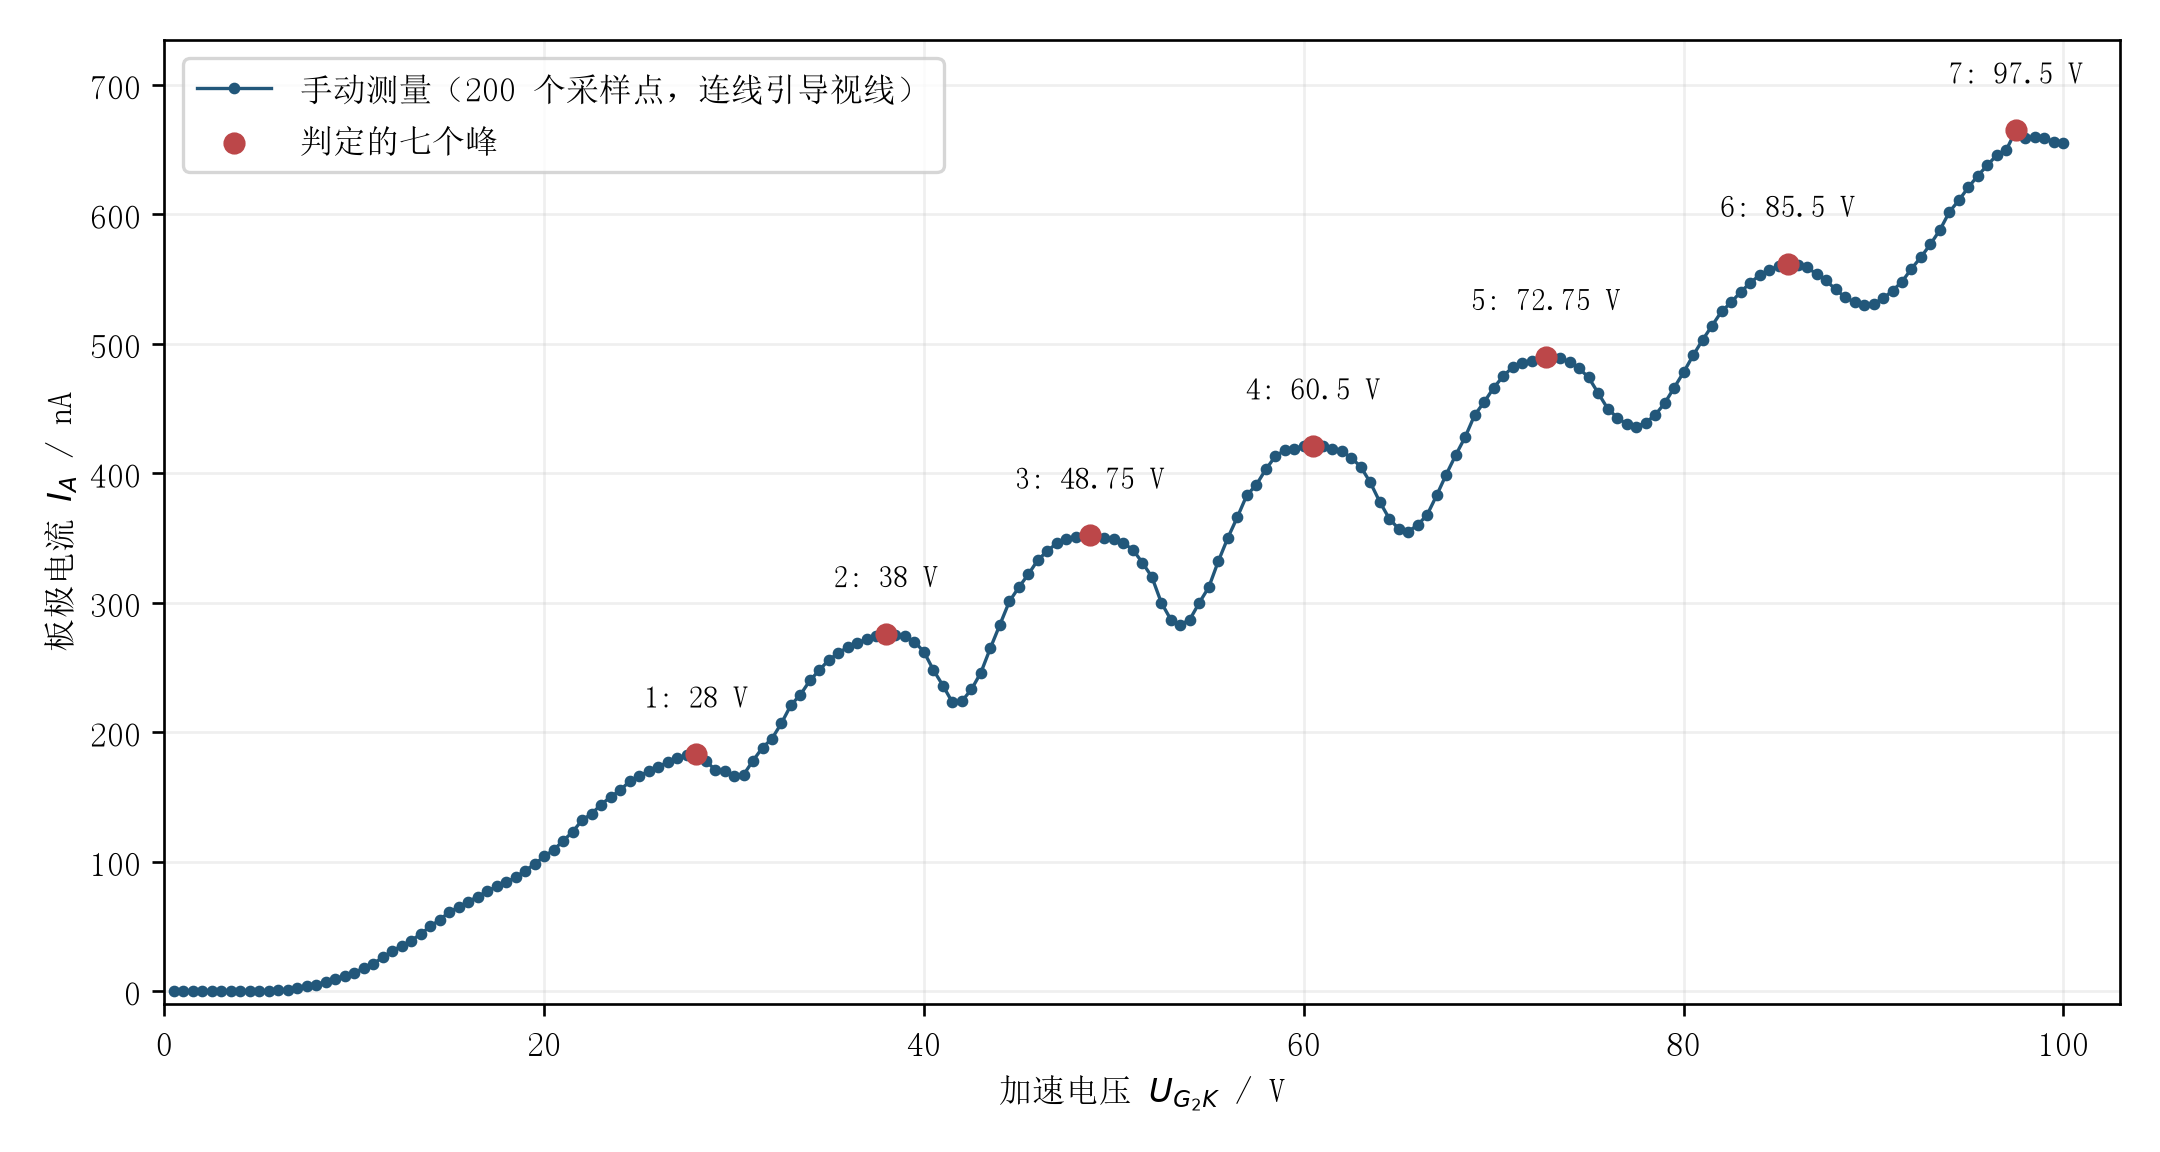
\includegraphics[width=\linewidth,height=.47\textheight,keepaspectratio]{../assets/manual_curve.png}
\caption{手动电流—电压曲线与判定的七个峰}
\end{figure}

低压段电流接近零，随后逐渐上升，在约 28 V 后开始呈现明显的峰谷。各峰的电流基线随电压总体上升，对有单个最大采样点的峰，采用该点的电压；若相邻多个采样点的电流同为最大值，则保留峰顶区间，以区间中点作为代表峰位。

\begin{center}
\begin{minipage}{\linewidth}
\centering

{\small
\setlength{\tabcolsep}{6pt}
\renewcommand{\arraystretch}{1.15}
\begin{tabular}{cccc}
\toprule

峰序 $n$ & 最大值所在电压/V & 代表峰位 $U_n$/V & 峰电流/nA \\

\midrule

1 & 28.0 & 28.00 & 183 \\

2 & 38.0 & 38.00 & 276 \\

3 & 48.5—49.0 & 48.75 & 352 \\

4 & 60.0—61.0 & 60.50 & 421 \\

5 & 72.5—73.0 & 72.75 & 490 \\

6 & 85.5 & 85.50 & 562 \\

7 & 97.5 & 97.50 & 665 \\

\bottomrule

\end{tabular}
}

\end{minipage}
\end{center}

\subsection*{2. 峰序—峰位线性拟合}

按课堂要求，对每组七个峰分别作普通最小二乘线性拟合：

\begin{equation}
U_n=A+n\Delta U,\qquad n=1,\ldots,7.
\end{equation}

其中 $\Delta U$ 是拟合斜率，代表相邻峰的平均电压间隔，作为本次测得的有效激发电势；$A$ 是拟合截距，吸收接触电势、拒斥筛选及峰序定义等引起的整体偏移。
令 $\bar n=4$、$\bar U=N^{-1}\sum U_n$，定义中心化和量

\begin{equation}
S_{nn}=\sum(n-\bar n)^2=28,
\quad S_{UU}=\sum(U_n-\bar U)^2,
\quad S_{nU}=\sum(n-\bar n)(U_n-\bar U).
\end{equation}

则

\begin{equation}
\Delta U=\frac{S_{nU}}{S_{nn}},\qquad
A=\bar U-\Delta U\bar n,\qquad
r=\frac{S_{nU}}{\sqrt{S_{nn}S_{UU}}}.
\end{equation}

本次三组峰位均使用 $N=7$，自由度为 $N-2=5$。下表保留计算中间位数用于复核，最终结果按不确定度修约。

\begin{center}
\begin{minipage}{\linewidth}
\centering

{\small
\setlength{\tabcolsep}{6pt}
\renewcommand{\arraystretch}{1.15}
\begin{tabular}{ccccc}
\toprule

数据组 & $A$/V & $\Delta U$/V & 相关系数 $r$ & $R^2$ \\

\midrule

自动前测 & 14.27143 & 11.87143 & 0.999004 & 0.998008 \\

手动测量 & 14.78571 & 11.69643 & 0.999217 & 0.998434 \\

自动后测 & 14.25714 & 11.86786 & 0.998984 & 0.997969 \\

\bottomrule

\end{tabular}
}

\end{minipage}
\end{center}

三条拟合式为

\begin{equation}
\begin{aligned}
U_n^{\text{前}}/\mathrm V&=14.27143+11.87143n,\\
U_n^{\text{手}}/\mathrm V&=14.78571+11.69643n,\\
U_n^{\text{后}}/\mathrm V&=14.25714+11.86786n.
\end{aligned}
\end{equation}

\begin{figure}[H]
\centering
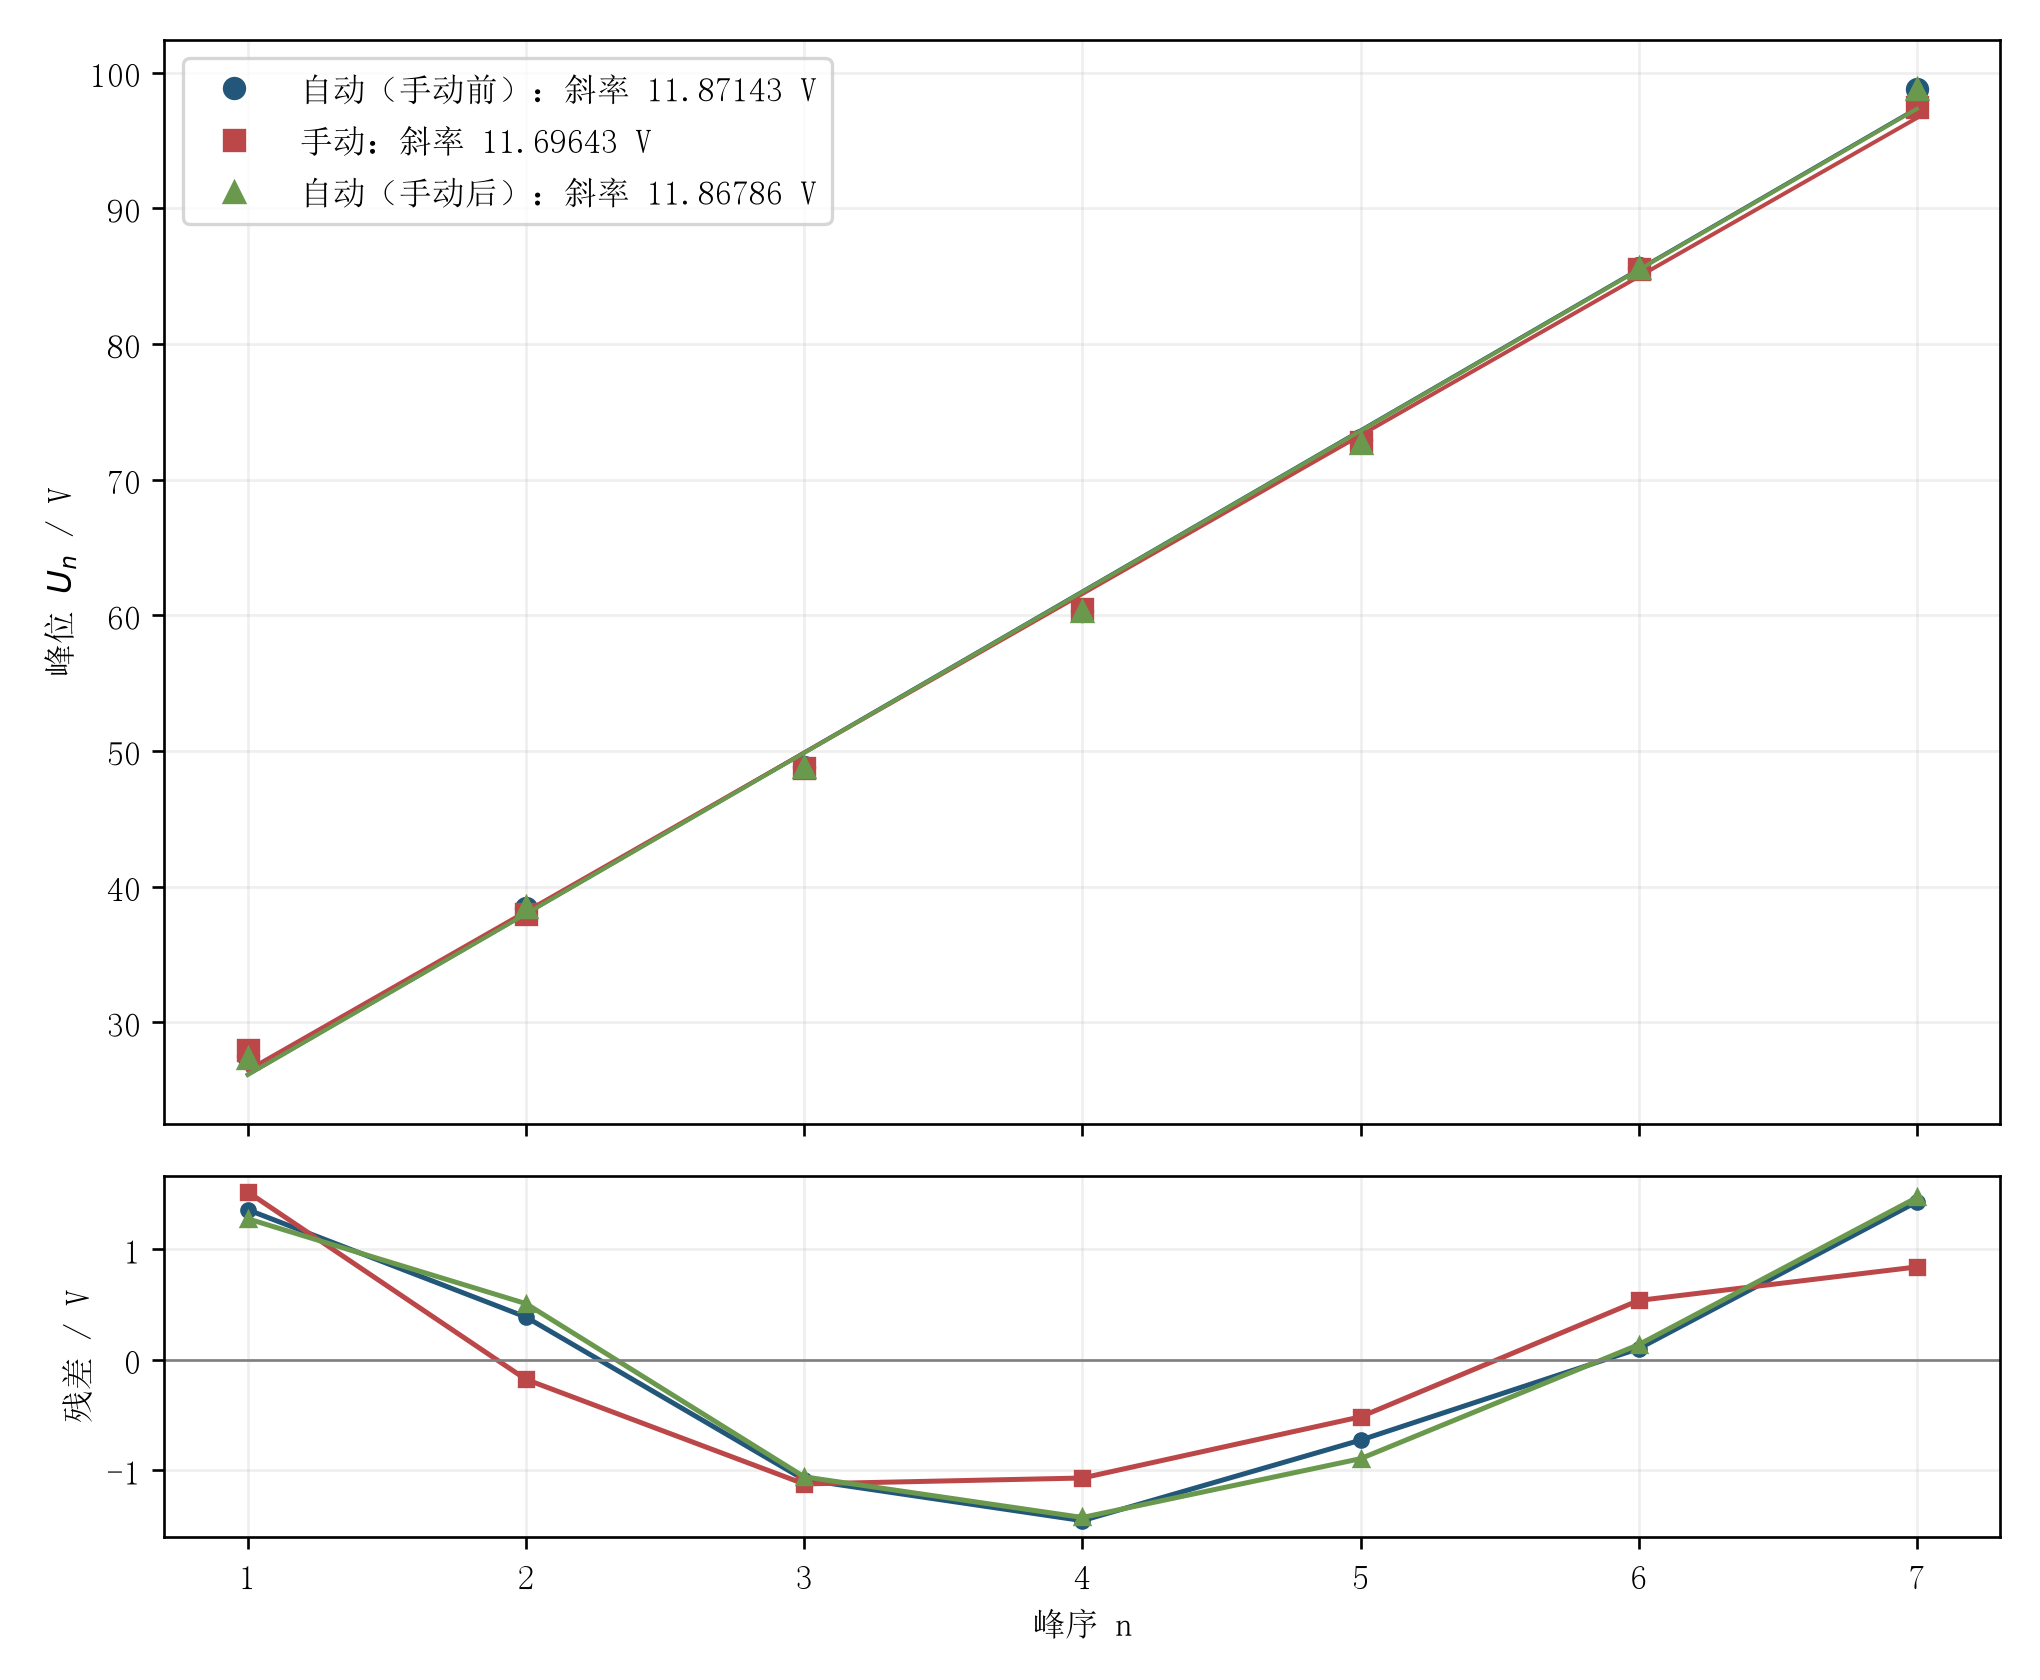
\includegraphics[width=\linewidth,height=.47\textheight,keepaspectratio]{../assets/peak_linear_fit.png}
\caption{三组峰位的线性拟合及残差}
\end{figure}

\begin{enumerate}
\item 三组相关系数均大于 0.998，峰位随峰序近似线性增加，支持激发能量具有确定的尺度。
\item 残差并非完全随机，自动的两组在两端偏正、中间偏负，均有约 1.4 V 的偏离，说明峰间距还有随峰序变化的趋势。
\item 较大的 $r$ 主要说明整体线性关系强，效果较理想。
\end{enumerate}

\subsection*{3. 斜率标准不确定度与结果表达}

课上给出由相关系数计算斜率标准不确定度的方法：

\begin{equation}
u(\Delta U)=|\Delta U|\sqrt{\frac{1/r^2-1}{N-2}}.
\end{equation}

计算得出：

\begin{center}
\begin{minipage}{\linewidth}
\centering

{\small
\setlength{\tabcolsep}{6pt}
\renewcommand{\arraystretch}{1.15}
\begin{tabular}{cccc}
\toprule

数据组 & 残差平方和/V\textsuperscript{2} & $u(\Delta U)$/V & 相对标准不确定度 \\

\midrule

自动前测 & 7.874286 & 0.237160 & 2.00\% \\

手动测量 & 6.008929 & 0.207174 & 1.77\% \\

自动后测 & 8.025357 & 0.239424 & 2.02\% \\

\bottomrule

\end{tabular}
}

\end{minipage}
\end{center}

保留两位有效数字，正式结果为：

\begin{equation}
\boxed{\Delta U_{\text{前}}=(11.87\pm0.24)\ \mathrm V},
\end{equation}

\begin{equation}
\boxed{\Delta U_{\text{手}}=(11.70\pm0.21)\ \mathrm V},
\end{equation}

\begin{equation}
\boxed{\Delta U_{\text{后}}=(11.87\pm0.24)\ \mathrm V}.
\end{equation}

未知电压表和微电流测量的允许误差限，因此不评定 B 类分量。

\subsection*{4. 与参考值比较}

采用实验教材附录使用的有效激发电势 $U_{\text{ref}}=11.61\ \mathrm V$ 作为比较值。

\begin{equation}
\delta=\frac{|\Delta U-11.61\ \mathrm V|}{11.61\ \mathrm V}\times100\%.
\end{equation}

\begin{center}
\begin{minipage}{\linewidth}
\centering

{\small
\setlength{\tabcolsep}{6pt}
\renewcommand{\arraystretch}{1.15}
\begin{tabular}{ccc}
\toprule

数据组 & $\Delta U$/V（未修约） & 相对误差 \\

\midrule

自动前测 & 11.87143 & 2.25\% \\

手动测量 & 11.69643 & 0.74\% \\

自动后测 & 11.86786 & 2.22\% \\

\bottomrule

\end{tabular}
}

\end{minipage}
\end{center}

\subsection*{5. 误差分析}

\subsubsection*{5.1 温度漂移与前后自动测量}

手动测量之后我发现在相等第二栅压的情况下，手动挡测得的电流平均比最初自动挡测得的电流小22\%，思考后认为是因为手动测量耗时较长，装置持续工作时的温度漂移可能改变热电子发射和空间电荷分布，影响电流大小及峰谷形状。

因此，我在手动测量后再进行了一次自动测量作对照。发现后一次自动测量的峰值电流与手动测量的峰值电流大小基本一致，所以基本可以确认是因为手动挡操作时间长，仪器温度上升导致的误差。
但是，每一次测量算出的激发电势与参考值的相对误差都控制在2.25\%以内，都是有效的测量。

\subsubsection*{5.2 峰位判定与采样步长}

手动峰顶较宽，第 3、4、5 峰出现平顶，精确极值不一定落在采样点上。取平均值是折中的方法，却仍然无法避免测量误差。

\subsubsection*{5.3 读数稳定性}

手动挡各点第二栅压电压需要手动调整，可能存在微小差别导致测量误差。同时，如果在电流示数没有稳定时过早读数，也会导致测量误差。
